% Options for packages loaded elsewhere
\PassOptionsToPackage{unicode}{hyperref}
\PassOptionsToPackage{hyphens}{url}
%
\documentclass[
  man,floatsintext]{apa6}
\usepackage{amsmath,amssymb}
\usepackage{lmodern}
\usepackage{iftex}
\ifPDFTeX
  \usepackage[T1]{fontenc}
  \usepackage[utf8]{inputenc}
  \usepackage{textcomp} % provide euro and other symbols
\else % if luatex or xetex
  \usepackage{unicode-math}
  \defaultfontfeatures{Scale=MatchLowercase}
  \defaultfontfeatures[\rmfamily]{Ligatures=TeX,Scale=1}
\fi
% Use upquote if available, for straight quotes in verbatim environments
\IfFileExists{upquote.sty}{\usepackage{upquote}}{}
\IfFileExists{microtype.sty}{% use microtype if available
  \usepackage[]{microtype}
  \UseMicrotypeSet[protrusion]{basicmath} % disable protrusion for tt fonts
}{}
\makeatletter
\@ifundefined{KOMAClassName}{% if non-KOMA class
  \IfFileExists{parskip.sty}{%
    \usepackage{parskip}
  }{% else
    \setlength{\parindent}{0pt}
    \setlength{\parskip}{6pt plus 2pt minus 1pt}}
}{% if KOMA class
  \KOMAoptions{parskip=half}}
\makeatother
\usepackage{xcolor}
\usepackage{graphicx}
\makeatletter
\def\maxwidth{\ifdim\Gin@nat@width>\linewidth\linewidth\else\Gin@nat@width\fi}
\def\maxheight{\ifdim\Gin@nat@height>\textheight\textheight\else\Gin@nat@height\fi}
\makeatother
% Scale images if necessary, so that they will not overflow the page
% margins by default, and it is still possible to overwrite the defaults
% using explicit options in \includegraphics[width, height, ...]{}
\setkeys{Gin}{width=\maxwidth,height=\maxheight,keepaspectratio}
% Set default figure placement to htbp
\makeatletter
\def\fps@figure{htbp}
\makeatother
\setlength{\emergencystretch}{3em} % prevent overfull lines
\providecommand{\tightlist}{%
  \setlength{\itemsep}{0pt}\setlength{\parskip}{0pt}}
\setcounter{secnumdepth}{-\maxdimen} % remove section numbering
% Make \paragraph and \subparagraph free-standing
\ifx\paragraph\undefined\else
  \let\oldparagraph\paragraph
  \renewcommand{\paragraph}[1]{\oldparagraph{#1}\mbox{}}
\fi
\ifx\subparagraph\undefined\else
  \let\oldsubparagraph\subparagraph
  \renewcommand{\subparagraph}[1]{\oldsubparagraph{#1}\mbox{}}
\fi
\ifLuaTeX
\usepackage[bidi=basic]{babel}
\else
\usepackage[bidi=default]{babel}
\fi
\babelprovide[main,import]{english}
% get rid of language-specific shorthands (see #6817):
\let\LanguageShortHands\languageshorthands
\def\languageshorthands#1{}
% Manuscript styling
\usepackage{upgreek}
\captionsetup{font=singlespacing,justification=justified}

% Table formatting
\usepackage{longtable}
\usepackage{lscape}
% \usepackage[counterclockwise]{rotating}   % Landscape page setup for large tables
\usepackage{multirow}		% Table styling
\usepackage{tabularx}		% Control Column width
\usepackage[flushleft]{threeparttable}	% Allows for three part tables with a specified notes section
\usepackage{threeparttablex}            % Lets threeparttable work with longtable

% Create new environments so endfloat can handle them
% \newenvironment{ltable}
%   {\begin{landscape}\centering\begin{threeparttable}}
%   {\end{threeparttable}\end{landscape}}
\newenvironment{lltable}{\begin{landscape}\centering\begin{ThreePartTable}}{\end{ThreePartTable}\end{landscape}}

% Enables adjusting longtable caption width to table width
% Solution found at http://golatex.de/longtable-mit-caption-so-breit-wie-die-tabelle-t15767.html
\makeatletter
\newcommand\LastLTentrywidth{1em}
\newlength\longtablewidth
\setlength{\longtablewidth}{1in}
\newcommand{\getlongtablewidth}{\begingroup \ifcsname LT@\roman{LT@tables}\endcsname \global\longtablewidth=0pt \renewcommand{\LT@entry}[2]{\global\advance\longtablewidth by ##2\relax\gdef\LastLTentrywidth{##2}}\@nameuse{LT@\roman{LT@tables}} \fi \endgroup}

% \setlength{\parindent}{0.5in}
% \setlength{\parskip}{0pt plus 0pt minus 0pt}

% Overwrite redefinition of paragraph and subparagraph by the default LaTeX template
% See https://github.com/crsh/papaja/issues/292
\makeatletter
\renewcommand{\paragraph}{\@startsection{paragraph}{4}{\parindent}%
  {0\baselineskip \@plus 0.2ex \@minus 0.2ex}%
  {-1em}%
  {\normalfont\normalsize\bfseries\itshape\typesectitle}}

\renewcommand{\subparagraph}[1]{\@startsection{subparagraph}{5}{1em}%
  {0\baselineskip \@plus 0.2ex \@minus 0.2ex}%
  {-\z@\relax}%
  {\normalfont\normalsize\itshape\hspace{\parindent}{#1}\textit{\addperi}}{\relax}}
\makeatother

% \usepackage{etoolbox}
\makeatletter
\patchcmd{\HyOrg@maketitle}
  {\section{\normalfont\normalsize\abstractname}}
  {\section*{\normalfont\normalsize\abstractname}}
  {}{\typeout{Failed to patch abstract.}}
\patchcmd{\HyOrg@maketitle}
  {\section{\protect\normalfont{\@title}}}
  {\section*{\protect\normalfont{\@title}}}
  {}{\typeout{Failed to patch title.}}
\makeatother

\usepackage{xpatch}
\makeatletter
\xapptocmd\appendix
  {\xapptocmd\section
    {\addcontentsline{toc}{section}{\appendixname\ifoneappendix\else~\theappendix\fi\\: #1}}
    {}{\InnerPatchFailed}%
  }
{}{\PatchFailed}
\usepackage{csquotes}
\ifLuaTeX
  \usepackage{selnolig}  % disable illegal ligatures
\fi
\IfFileExists{bookmark.sty}{\usepackage{bookmark}}{\usepackage{hyperref}}
\IfFileExists{xurl.sty}{\usepackage{xurl}}{} % add URL line breaks if available
\urlstyle{same} % disable monospaced font for URLs
\hypersetup{
  pdftitle={Perception of lexical pitch accent in South Kyungsang Korean},
  pdfauthor={Hyunjung Joo1},
  pdflang={en-EN},
  hidelinks,
  pdfcreator={LaTeX via pandoc}}

\title{Perception of lexical pitch accent in South Kyungsang Korean}
\author{Hyunjung Joo\textsuperscript{1}}
\date{}


\shorttitle{QP1}

\authornote{

Correspondence concerning this article should be addressed to Hyunjung Joo. E-mail: \href{mailto:hyunjung.joo@rutgers.edu}{\nolinkurl{hyunjung.joo@rutgers.edu}}

}

\affiliation{\vspace{0.5cm}\textsuperscript{1} Rutgers University}

\begin{document}
\maketitle

\hypertarget{brief-introduction}{%
\subsection{1. Brief introduction}\label{brief-introduction}}

The goal of the present study is to understand how continuous f0 contour is stored in our phonological representation and what kind of phonetic correlates of f0 contour can be defined as distinctive phonological units in the intonational grammar. Specifically, the present study will examine how South Kyungsang Korean listeners perceive their lexical pitch accents, H vs.~LH, by looking at different theoretical approaches to the phonological representation of f0 contour: AM vs.~Configurational/TCoG approach. These two types of the approaches will provide an understanding of whether several specific turning points phonologically represent continuous f0 contour or the configurations of f0 contour as a whole functions as primitive units of f0 contour. The AM approach abstracts away from the phonetic details such as overall contour shapes to the particular tonal targets. Relevant acoustic correlates for H vs.~LH distinction under the AM theory can be f0 peak alignment and the existence of L target. In contrast, the TCoG approach accounts for various phonetic details such as rise shape as well as the turning points. From the f0 contour of actual production in SKK above, we have seen various phonetic aspects that can characterize H vs.~LH pitch accents. Among these perceptual cues, how can we account for the phonological representation of the lexical pitch accent in SKK under these two theoretical approaches?

In order to test the two theories above, a perception experiment was designed to see the impact of f0 peak alignment and rise shape. Recorded sounds were first obtained from a female SKK speaker and then were manipulated depending on the peak alignment and the rise shape in Praat. In a two-alternative forced choice task, listeners of SKK were asked to choose a visual stimulus that matches with the resynthesized sound stimulus. Based on their responses, results were statistically analyzed to see which hypothesis can be supported.

\hypertarget{methods}{%
\subsection{2. Methods}\label{methods}}

\hypertarget{stimuli}{%
\subsection{2.1. Stimuli}\label{stimuli}}

Target words consisted of three monosyllabic homophone pairs (\emph{gan} {[}kan{]} (`taste' and `liver'), \emph{bam} {[}pam{]} (`night' and `chestnut'), \emph{bal} {[}pal{]} (`foot' and `shade')), contrasting by lexical pitch accent (H vs.~LH) as shown in Table 1. Filler words consisted of ten monosyllabic words (\emph{/gam/, /gang/, /bang/, /bang/, /dan/, /nan/, /nam/, /dam/, /kal/, /dal/}), which differ in either onset or coda from the target words as shown in Table 2. Both the target and the filler words (test words) were embedded in a carrier sentence, `Click black \_\_\_ with the mouse this time', in an IP-medial position. The test words were always preceded by the word \emph{kkamansaeg} (`black') to derive the preceding context as H+L. Since LH tone always initiates rising from the low f0 value, the contours for both H and LH tone were designed to initiate rising from the same low f0 value, by making the preceding context end with L tone for a fair comparison. 15 repetitions of these sentences were recorded by a female SKK speaker in a sound-proof booth in Seoul, South Korea, using a SHURE KSM44A microphone. In order to clearly induce the tonal contrast, she was asked to assign a contrastive focus on the test words with a normal speech rate. Note that in South Kyungsang Korean, only one pitch accent survives in an accentual phrase (AP), while the other pitch accents in the AP become deaccented (Kim \& Jun 2009). Hence, a contrastive focus was assigned onto the target word in the AP-medial position, in order to see the lexical pitch accent clearly. Prosodic rendition of the recorded utterances was checked by a trained K-ToBI (Korean TOnes and Break Indices, Jun 2000) transcriber. The f0 contours of the recorded utterances are provided in Figure 1.

\newpage

\begin{table}[H]

\caption{\label{tab:table1}Three monosyllabic homophone pairs.}
\centering
\begin{tabular}[t]{l|l|l}
\hline
Word & Tone & Meaning\\
\hline
/kan/ & H & taste\\
\hline
/kan/ & LH & liver\\
\hline
/pam/ & H & night\\
\hline
/pam/ & LH & chestnut\\
\hline
/pal/ & H & foot\\
\hline
/pal/ & LH & shade\\
\hline
\end{tabular}
\end{table}
\begin{figure}

{\centering 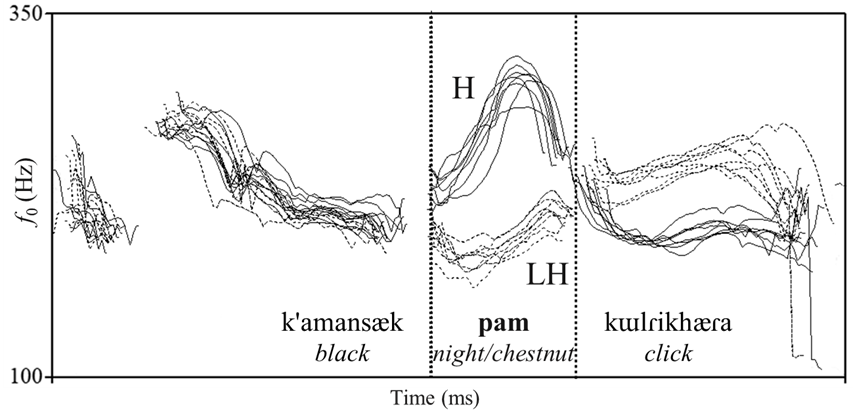
\includegraphics[width=0.9\linewidth]{images/picture1} 

}

\caption{f0 contours of the target words (/pam/ with H and LH tone) in an embedded sentence recorded by a female SKK speaker.}\label{fig:picture1}
\end{figure}

Based on the recorded utterances above, several basic landmarks that consist of f0 rising contour for both H and LH such as starting and peak points were measured as shown in Figure 2. The f0 values of these landmarks were then used as baseline values for the sound manipulation. First, f0 minimum values were extracted from the L target of the target word (b) and the preceding word (a). Next, f0 maximum values were obtained from the H target of the target word (c). Lastly, duration of the target word was measured from the onset of consonant release to the offset of the rime (d). These values were averaged across 15 repetitions (10) and were used for the stimulus resynthesis. To manipulate \emph{peak alignment} and \emph{rising shape} of f0 contour for the target word, a pitch stylizing function was used in Praat (Boersma \& Weenink 2009). The pitch stylizing function simplifies a continuous pitch curve into several pitch points and enables us to modify the pitch values manually.

\begin{figure}[H]

{\centering 
\includegraphics[width=0.9\linewidth]{images/picture2} 

}

\caption{Baseline values for stimulus resynthesis. The f0 value for (a) marks a L target (f0 minimum) of the preceding word and the  f0 value for (b) marks a L target (f0 minimum) of the target word. The f0 value for (c) indicates a H target (f0 maximum) of the target word. (d) indicates the duration of the target word from the onset of consonant release to the offset of the rime.}\label{fig:picture2}
\end{figure}
\newpage

\hypertarget{stimulus-resynthesis}{%
\subsection{2.2. Stimulus resynthesis}\label{stimulus-resynthesis}}

\hypertarget{manipulation-of-peak-alignment}{%
\subsection{\texorpdfstring{2.2.1. Manipulation of \emph{peak alignment}}{2.2.1. Manipulation of peak alignment}}\label{manipulation-of-peak-alignment}}

First, to test how f0 peak alignment plays a role in SKK listeners' perception, peak alignment was adjusted as illustrated in Figure 3. Segmental duration was set to be ambiguous, with the mean duration of all H and LH words (290 ms for /kan/, 252 ms for /pal/, and 280 ms for /pam/). However, the timing of peak alignment was varied from 20\%, 40\%, 60\%, 80\% to 100\% of the rime duration, resulting in 5 steps. Each alignment step was increased with 20\% of the rime duration (50 ms for /kan/, 46 ms for /pal/, 48 ms for /pam/). As for the f0 value of the target word, it started with 210 Hz and increased up to 270 Hz to reach its H target (f0 peak). After reaching its target, the f0 value ended with 210 Hz. The f0 rising contour shape remained the same but only the timing of the f0 contour differed along the continuum. The f0 value of the preceding HL tone ended with the same f0 value (210 Hz) as at the vowel onset of the target words.

\begin{figure}[H]

{\centering 
\includegraphics[width=0.7\linewidth]{images/picture3} 

}

\caption{Manipulation of peak alignment. Step 1 indicates earlier peaks, while Step 5 indicates later peaks.}\label{fig:picture3}
\end{figure}

\newpage

\hypertarget{manipulation-of-rise-shape}{%
\subsection{\texorpdfstring{2.2.2. Manipulation of \emph{rise shape}}{2.2.2. Manipulation of rise shape}}\label{manipulation-of-rise-shape}}

Next, to test whether f0 rise shape matters in the pitch accent categorization of SKK, f0 rise shape was manipulated as shown in Figure 4. As for the target word, the f0 value of the rising contour started from the vowel onset (210 Hz), and it ended at the offset of the sonorant coda (270 Hz). In order to create convex and concave rise shapes, the f0 value at the midpoint of the rime was increased by 10 Hz steps from 215 Hz to 265 Hz, resulting in 5 steps. Thus, for the most convex shape, the f0 value started with 210 Hz, increased by 5 Hz at the vowel midpoint, and then reached its H target with 270 Hz. For the most concave shape, the f0 value started 210 Hz, but increased greater by 65 Hz at the vowel midpoint, and then reached its H target with 270 Hz. Adjusting the f0 value at the midpoint made it possible to make either scooped or domed shape. The f0 value of the preceding HL tone ended at the same level (210 Hz) as the vowel onset of the target word. Segmental duration was ambiguous, with mean duration of all H and LH words (290 ms for /kan/, 252 ms for /pal/, and 280 ms for /pam/).

\begin{figure}[H]

{\centering 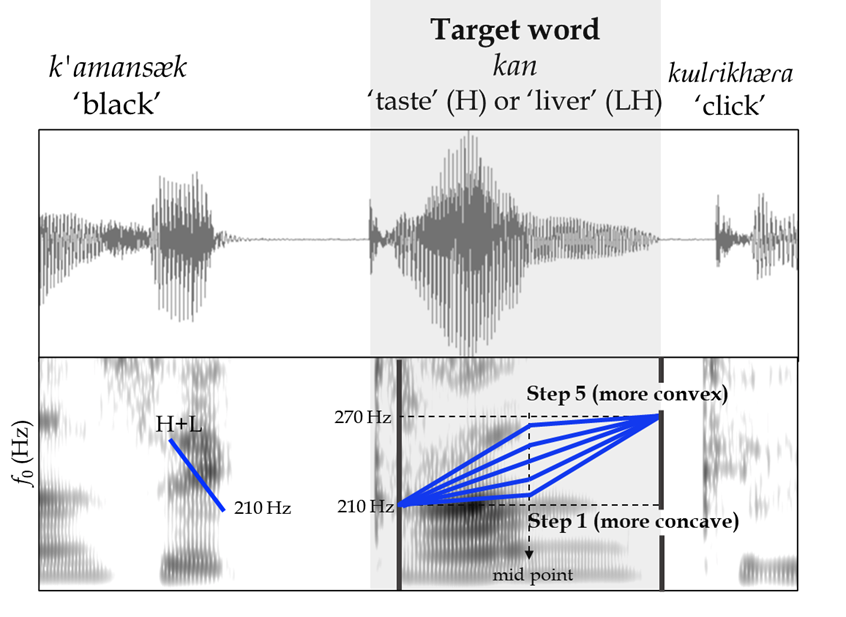
\includegraphics[width=0.7\linewidth]{images/picture4} 

}

\caption{Manipulation of rise shape. Step 1 indicates more concave f0 shapes, while Step 5 indicates more convex shapes.}\label{fig:picture4}
\end{figure}

\hypertarget{participants}{%
\subsection{2.3. Participants}\label{participants}}

22 native listeners of South Kyungsang Korean (11 females, 11 males) participated in the perception experiment. They were aged from 20 to 28 (mean = 23.33), born and raised in the southern part of the Kyungsang region, mainly Pusan and neighboring cities in South Korea. In order to avoid any dialectal influence, the participants' parents were also born and raised in the South Kyungsang region. None of them had hearing problems and they were compensated for their participation.

\hypertarget{procedure}{%
\subsection{2.4. Procedure}\label{procedure}}

Participants saw visual stimuli through a laptop and heard sound stimuli using a headphone (Sony MDR-7509) in a sound-proof booth in Ulsan, South Korea. A two-alternative forced choice experiment was carried out using Psychopy (Peirce 2009). Before the experimental session, the participants had a short training session to become familiarized with the experimental settings. In the main experiment, for each trial, they were asked to look at the visual stimuli on the screen upon hearing the sound stimuli and responded by pressing the button of the visual target that matched the target word. Visual stimuli were presented with two different images for a homophone pair (e.g., for the word /pam/, `night' on the left and `chestnut' on the right for /pam/) on the screen, as shown in Figure 5. In each task, 120 target were used to see the effect of \emph{peak alignment} and \emph{rise shape}: 2 factors (5 f0 peak alignments + 5 f0 rise shapes) x 3 items (/kan/ for taste and liver, /pam/ for night and chestnut, /pal/ for foot and shade) x 4 repetitions. In order to mask the purpose of this study, 180 filler stimuli were added: the combinations of the target words and 10 items differing either onset or coda from the target words (/kam/, /kang/, /pan/, /pang/, /tan/, /nan/, /nam/, /tam/, /khal/, /tal/). A total of 300 stimuli were presented in the study. The four blocks (repetitions) were presented in a randomized order, with an interval between the blocks (1st interval: 30 sec, 2nd interval: 5 mins, and 3rd interval: 30 sec). Among the 22 subjects, one participant was excluded due to the wrong responses.

\begin{figure}[H]

{\centering 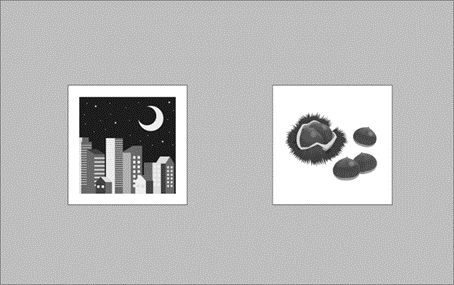
\includegraphics[width=1\linewidth]{images/picture5} 

}

\caption{A screenshot of the visual stimuli.}\label{fig:picture5}
\end{figure}

\hypertarget{measurement-and-statistical-analysis}{%
\subsection{2.5. Measurement and statistical analysis}\label{measurement-and-statistical-analysis}}

In order to see how SKK listeners perceive f0 contours depending on \emph{rise shape} and \emph{peak alignment}, responses for each step in the continuum were collected. Then, a series of a generalized linear mixed effects model with a binomial linking function were carried out using the lme4 package in R (R Core Team 2018), separately for the \emph{Peak alignment} and the \emph{Rise shape} data. To examine the effects of these factors on the identification of pitch accents, \emph{responses} (H vs.~LH) were used as a dependent variable. H responses were coded as 1, and LH responses were coded as 0. The models included Continuum steps for \emph{Peak alignment} (5 steps from earlier to later peaks) and \emph{Rise shape} (5 steps from concave to convex shapes) as a fixed effect. The fixed effects were included as continuous variables. Due to convergence failure, random intercepts and slopes were included in order to keep maximal random structures (Barr, Levy, Scheepers \& Tily 2013). As for the Continuum steps for \emph{Rise shape}, random intercept and slope were set for both \emph{Subject} (10F, 11M) and \emph{Item} (/kan/, /pal/, /pam/). As for Continuum steps for \emph{Rise shape}, random intercept was set for both \emph{Subject} and \emph{Item}, but random slope was set for either \emph{Subject} or \emph{Item}. Below are three logistic regression models used in this study, with \emph{Model 1} run for \emph{Peak alignment} and \emph{Model 2} run for \emph{Rise shape}. p-values less than .05 were reported as significant.

R code for mixed-effects logistic regression models

\begin{itemize}
\item
  \emph{Model 1}: \texttt{glmer\ (responses\ \textasciitilde{}\ steps\_peak\ +\ (1\ +\ steps\_peak\ \textbar{}\ subject)\ +\ (1\ +\ steps\_peak\ \textbar{}\ item),\ data\ =\ peak\_alignment)}
\item
  \emph{Model 2}: \texttt{glmer\ (responses\ \textasciitilde{}\ steps\_shape\ +\ (1\ +\ steps\_shape\ \textbar{}\ subject)\ +\ (1\ \textbar{}\ item),\ data\ =\ rise\_shape)}
\end{itemize}

\hypertarget{results}{%
\subsection{3. Results}\label{results}}

\hypertarget{peak-alignment}{%
\subsection{3.1. Peak alignment}\label{peak-alignment}}

Figure 6 shows the percentage of H responses for each step of the continuum from earlier to later peak alignments. Results showed that SKK listeners did not differentiate H vs.~LH depending on f0 peak alignment, regardless of whether the peak is aligned earlier or later. The H response percentage for all the Continuum steps for \emph{Peak alignment} was below chance level (mean = 0.16, sd = 0.37). In the glmer model, the Continuum steps for \emph{Peak alignment} did not show any statistical significance (b = -0.09, z = -0.89, p \textless.001), as shown in Table 3. That is, regardless of the timing of f0 peak, the listeners responded to all steps in the continuum mainly as LH.
\newpage

\begin{figure}[H]

{\centering 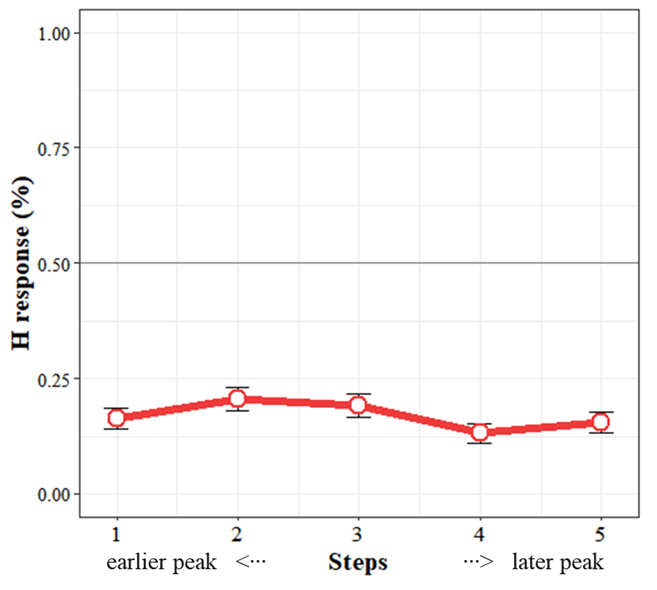
\includegraphics[width=1\linewidth]{images/picture6} 

}

\caption{H response percentage for Peak alignment. Towards Step 1 indicates earlier peak, while towards Step 5 indicates later peak.}\label{fig:picture6}
\end{figure}

\begin{table}[H]

\caption{\label{tab:table2}Statistical result of Peak alignment effect on tonal categorization.}
\centering
\begin{tabular}[t]{l|r|r|r|r}
\hline
Model 1 & Estimate & Std. Error & z value & Pr(>|z|)\\
\hline
(Intercept) & -1.643 & 0.364 & -4.509 & 0.000\\
\hline
peak & -0.090 & 0.102 & -0.890 & 0.373\\
\hline
\end{tabular}
\end{table}
\newpage

The pattern of the \emph{Peak alignment} effect on tonal categorization was further confirmed by examining the pattern by \emph{Item} and \emph{Subject}. Figure 7 displays the H response percentage for \emph{Peak alignment} by \emph{Item} (/kan/, /pal/, /pam/). The H response percentage for all Continuum steps for \emph{Peak alignment} was below chance level for the three lexical items (/kan/: mean = 0.17, sd = 0.38; /pal/: mean = 0.17, sd = 0.38; /pam/: mean = 0.17, sd = 0.37). There were no by-item effects on tonal categorization, indicating the absence of a \emph{Peak alignment} effect across items and subjects. Specifically, regardless of the timing of the f0 peak, the listeners responded as LH for all the continuum steps for the different lexical items (/kan/, /pal/, and /pam/).

\begin{figure}[H]

{\centering 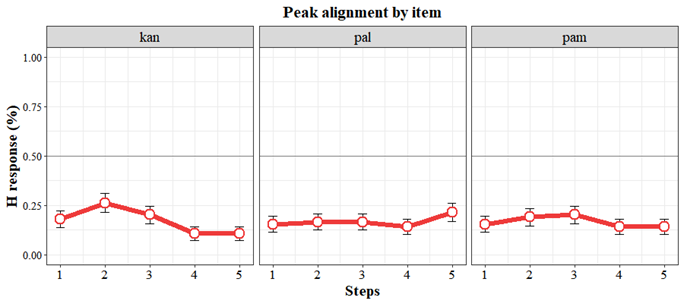
\includegraphics[width=1\linewidth]{images/picture7} 

}

\caption{H response percentage for Peak alignment. Towards Step 1 indicates earlier peak, while towards Step 5 indicates later peak.}\label{fig:picture7}
\end{figure}

Figure 8 displays the H response percentage for \emph{Peak alignment} by \emph{Subject}. The results indicated that for most subjects (19 out of 21), the H response percentage was below chance level, indicating that they did not distinguish H vs.~LH based on the earlier or later peaks of alignment. Four subjects (f07, f08, f00, M09) exhibited a tendency for later peaks to be more likely identified as LH tone, but still, all the steps were below chance level, indicating the absence of the \emph{Peak alignment} effect. Only two subjects (M04, M05) showed H response percentages above chance level at Step 4 and Step 5, respectively. However, the directionality of the response percentage was opposite from what was expected if they were to respond to the timing of the peak alignment. That is, their H response percentages increased from earlier to later peaks, indicating that the later peaks were identified as H tone, not LH tone, which supports the absence of the \emph{Peak alignment} effect. Thus, there were no individual differences in terms of the \emph{Peak alignment} effect on tonal categorization. Overall, the results of by-item and by-subject responses suggest that SKK listeners do not use \emph{Peak alignment} cues to distinguish H vs.~LH pitch accents.

\begin{figure}[H]

{\centering 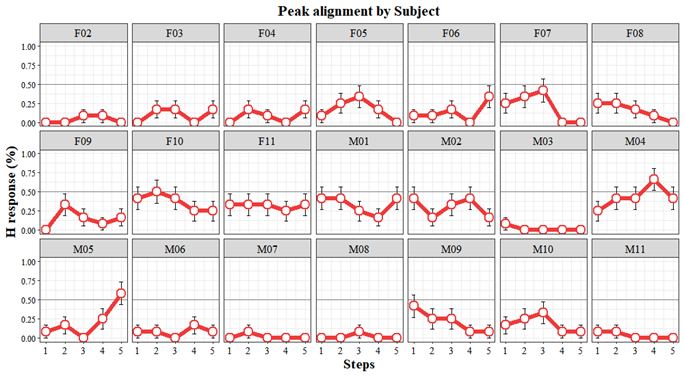
\includegraphics[width=1\linewidth]{images/picture8} 

}

\caption{H response percentage for Peak alignment by Item (/kan/, /pal/, /pam/). Towards Step 1 indicates earlier peak, while towards Step 5 indicates later peak.}\label{fig:picture8}
\end{figure}

\hypertarget{rise-shape}{%
\subsection{3.2. Rise shape}\label{rise-shape}}

Results showed to what extent SKK listeners categorically perceived H vs.~LH depending on \emph{Rise shape}, either concave or convex, in the continuum, as shown in Figure 9. The H response percentage for Rise shape showed a linear relationship. Specifically, the H response percentage gradually increased from Step 1 to Step 5, which found to be significant in the binomial regression analysis (Model 2, b = 0.68, z = -7.61, p \textless.001; Model 3, b = 0.63, z = 10.75, p \textless.001). The parameter estimates of the model indicated that a one unit increase in the continuum for \emph{Rise shape} yielded a change in the log odds of selecting H tone by 0.68, with a positive difference of 33\% in the probability of selecting H tone. The category boundary (50\% crossover point) was at Step 2, as shown in the vertical line of Figure 9. Note that below Step 2, when the rise is more concave, listeners were more likely to respond as LH, while above Step 2, when the rise is more convex, they were more likely to respond as H. At the two extremes of the continuum, listeners responded to Step 1 mainly as an LH tone (mean = 0.37, sd = 0.48), whereas they responded to Step 5 mainly as an H tone (mean = 0.85, sd = 0.35). Therefore, SKK listeners were able to differentiate H vs.~LH depending on the f0 rise shape, whether it is concave or convex.

\begin{figure}[H]

{\centering 
\includegraphics[width=1\linewidth]{images/picture9} 

}

\caption{H response percentage for Rise shape. Towards Step 1 indicates more concave shape, while towards Step 5 indicates more convex shape. }\label{fig:picture9}
\end{figure}

\begin{table}[H]

\caption{\label{tab:table3}Statistical result of Rise shape effect on tonal categorization.}
\centering
\begin{tabular}[t]{l|r|r|r|r}
\hline
Model 2 & Estimate & Std. Error & z value & Pr(>|z|)\\
\hline
(Intercept) & -1.362 & 0.293 & -4.649 & 0\\
\hline
shape & 0.689 & 0.091 & 7.612 & 0\\
\hline
\end{tabular}
\end{table}

Figure 10 shows the percentage of H response for \emph{Rise shape} by Item (/kan/, /pal/, /pam/). The H response percentage showed the same patterns across the three lexical items. The category boundary for all the items was at Step 2. The response percentage increased from Step 1 to Step 5, showing that the more concave shapes were perceived as LH, the more convex shapes were perceived as H. At the two extremes in the continuum, Step 1 was perceived as LH (/kan/: mean = 0.35, sd = 0.48; /pal/: mean = 0.37, sd = 0.49; /pam/: mean = 0.41, sd = 0.49), while Step 5 was perceived as H (/kan/: mean = 0.86, sd = 0.35; /pal/: mean = 0.81, sd = 0.40; /pam/: mean = 0.89, sd = 0.31). This by-item pattern further supports the effect of \emph{Rise shape} on SKK's tonal categorization.

\begin{figure}[H]

{\centering 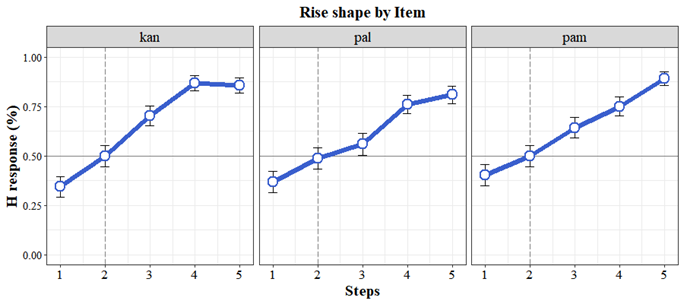
\includegraphics[width=1\linewidth]{images/picture10} 

}

\caption{H response percentage for Rise shape by Item (/kan/, /pal/, /pam/). Towards Step 1 indicates more concave shape, while towards Step 5 indicates more convex shape. }\label{fig:picture10}
\end{figure}
\newpage

Figure 11 shows the percentage of H response for \emph{Rise shape} by \emph{Subject}. Among the 21 subjects, 13 subjects with blue borders in Figure 11 (f02, f03, f06, f07, f09, f01, M01, M03, M05, M06, M08, M09, M10) showed a categorical boundary around Step 2 and 3. Below the categorical boundary, when the rise shape is concave, they responded as LH, while above it, when the rise shape is convex, they responded as H. The rest of the subjects without yellow borders in Figure 11 (f04, f05, f08, f10, M02, M04, M07, M11) showed a similar tendency to the overall response pattern, such that the concave shapes were more likely to be categorized as LH, while the convex shapes were categorized as H. Despite the similar tendency, all the response percentage was above chance level, showing that the listeners perceived all continuum steps as H tone. Nevertheless, it can still be concluded that the majority of SKK listeners used Rise shape as a perceptual cue to differentiate H vs.~LH tones.

\begin{figure}[H]

{\centering 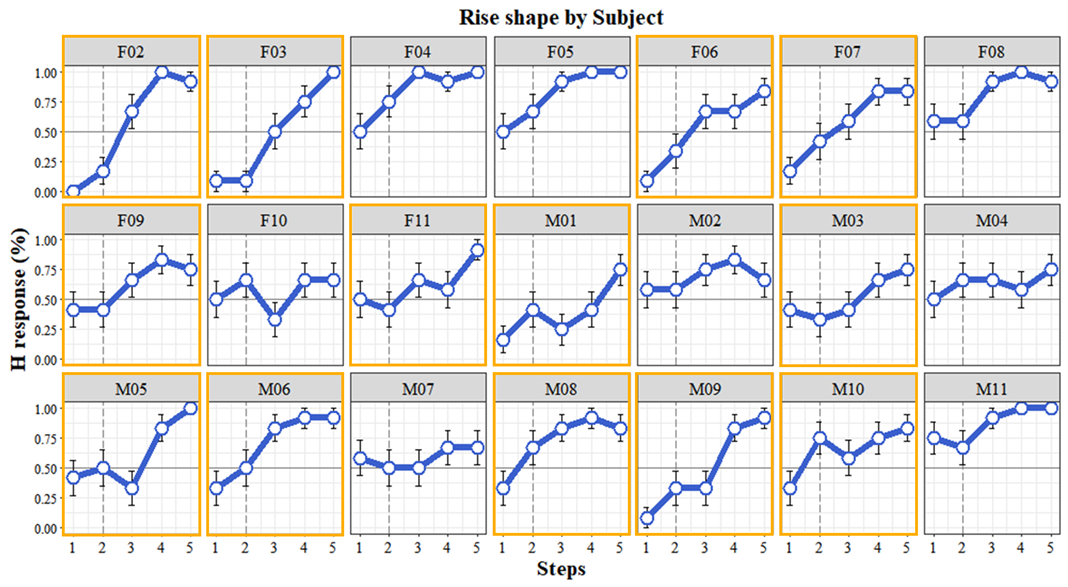
\includegraphics[width=1\linewidth]{images/picture11} 

}

\caption{H response percentage for Rise shape by Subject. Towards Step 1 indicates more concave shape, while towards Step 5 indicates more convex shape. }\label{fig:picture11}
\end{figure}


\end{document}
